% Created 2025-10-20 Mon 08:20
\documentclass[compress,dvipdfmx,11pt]{beamer}
\usepackage[T1]{fontenc}
\usepackage{graphicx}
\usepackage{amsmath}
\usepackage[normalem]{ulem}
\usepackage{hyperref}
\title[IA 研究会 @ 富山大]{\bf タイトル}
\author[]{XXX XXX, 大崎 博之}
\institute{関西学院大学 理工学部 情報科学科}
\date{2016 年 4 月 1 日}
\setlength{\parskip}{1.5ex}
\renewcommand{\textbf}{\alert}
\author{shun}
\date{\today}
\title{dummy}
\hypersetup{
 pdfauthor={shun},
 pdftitle={dummy},
 pdfkeywords={},
 pdfsubject={},
 pdfcreator={Emacs 28.2 (Org mode 9.5.5)}, 
 pdflang={Ja}}
\begin{document}

\tableofcontents

\newcommand{\pivec}{\mathbf \pi}
\newcommand{\xvec}{\mathbf x}
\newcommand{\yvec}{\mathbf y}
\newcommand{\zvec}{\mathbf z}
\newcommand{\Emat}{\mathbf E}
\newcommand{\Imat}{\mathbf I}

\bf

\section{はじめに}
\label{sec:org4de439a}

\subsection{研究の背景}
\label{sec:org2d7a159}

\begin{itemize}
\item あれが大事
\begin{itemize}
\item これも大事
\item そこでそれが必要
\end{itemize}
\item ところでこれは?
\begin{itemize}
\item あれも必要
\end{itemize}
\end{itemize}

\subsection{研究の目的}
\label{sec:org62060a1}

\begin{enumerate}
\item あれをする
\item それをする
\item それもする
\end{enumerate}
\begin{align}
T = \frac{MSS \, \sqrt{1.5}}{R \, \sqrt{p}}
\end{align}

\section{解析モデル}
\label{sec:org8cfe6a5}

\subsection{解析モデル}
\label{sec:org8142e08}

\begin{center}
\begin{center}
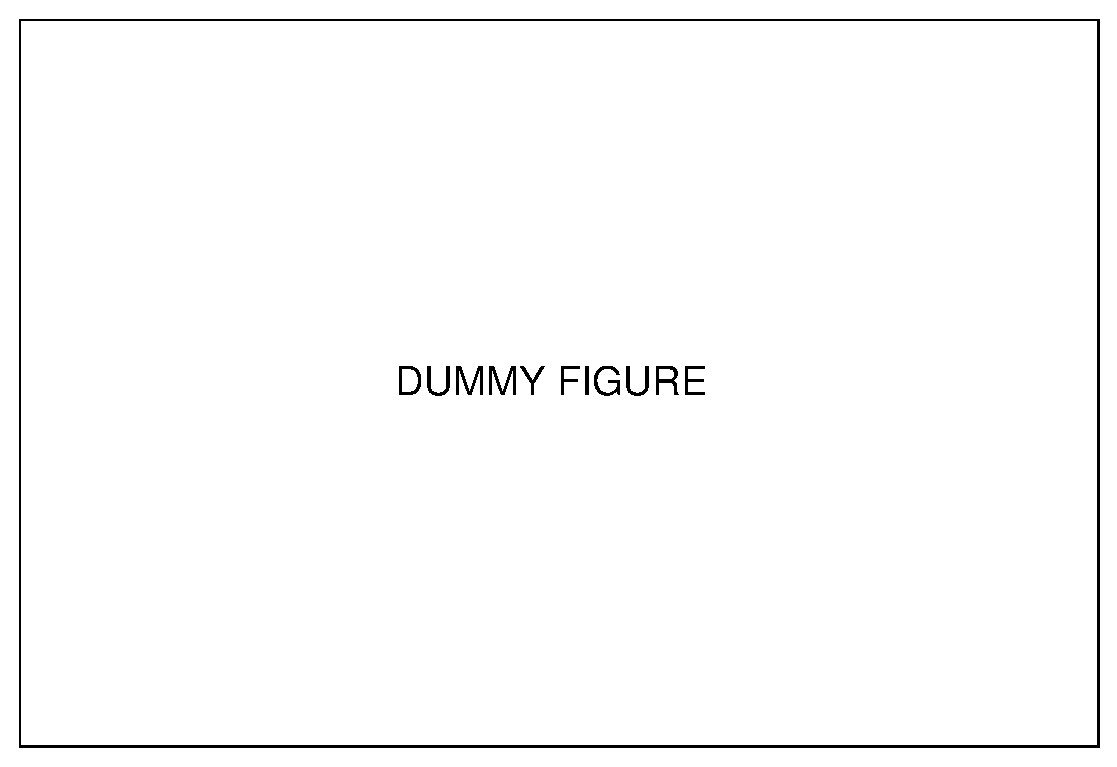
\includegraphics[width=\columnwidth]{./figure/dummy.eps}
\end{center}
\end{center}

\subsection{解析における仮定}
\label{sec:orgab1e645}

\begin{enumerate}
\item column\hfill{}\textsc{BMCOL}
\label{sec:org2ca8c45}
\begin{itemize}
\item \(T\): スループット
\begin{itemize}
\item あれを含む
\end{itemize}
\item \(R\): ラウンドトリップ時間
\begin{itemize}
\item 時間がたっても変化しない
\end{itemize}
\end{itemize}

\item column\hfill{}\textsc{BMCOL}
\label{sec:org36643b7}
\begin{itemize}
\item \(T\): スループット
\begin{itemize}
\item あれを含む
\end{itemize}
\item \(R\): ラウンドトリップ時間
\begin{itemize}
\item 時間がたっても変化しない
\end{itemize}
\end{itemize}
\end{enumerate}

\section{解析}
\label{sec:orga3ea564}

\subsection{キャッシュヒット率の導出}
\label{sec:org7c86458}

\begin{align}
T = \frac{MSS \, \sqrt{1.5}}{R \, \sqrt{p}}
\end{align}

\subsection{メッセージ配送遅延の導出}
\label{sec:orgd1e7870}

\begin{align}
T = \frac{MSS \, \sqrt{1.5}}{R \, \sqrt{p}}
\end{align}

\section{数値例}
\label{sec:org7b90d07}

\subsection{数値例: バッファサイズとスループットの関係}
\label{sec:org8cd67ae}

\begin{center}
\begin{center}
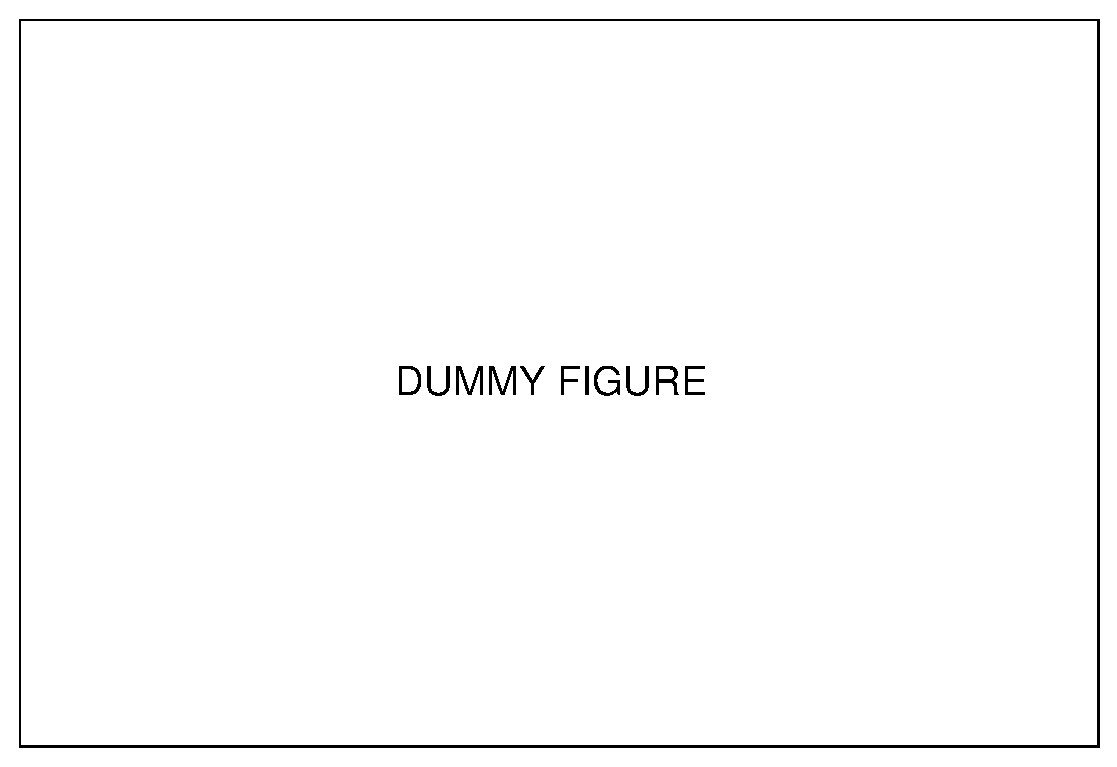
\includegraphics[width=.7\columnwidth]{./figure/dummy.eps}
\end{center}
\end{center}

\begin{center}
\(T\) = 12 [Mbit/s], \(B\) = 1,000 [byte], \(L\) = 1 [packet]
\end{center}

\subsection{数値例: バッファサイズとスループットの関係}
\label{sec:orgee77a50}

\begin{enumerate}
\item column\hfill{}\textsc{BMCOL}
\label{sec:org88d3156}
\begin{center}
\begin{center}
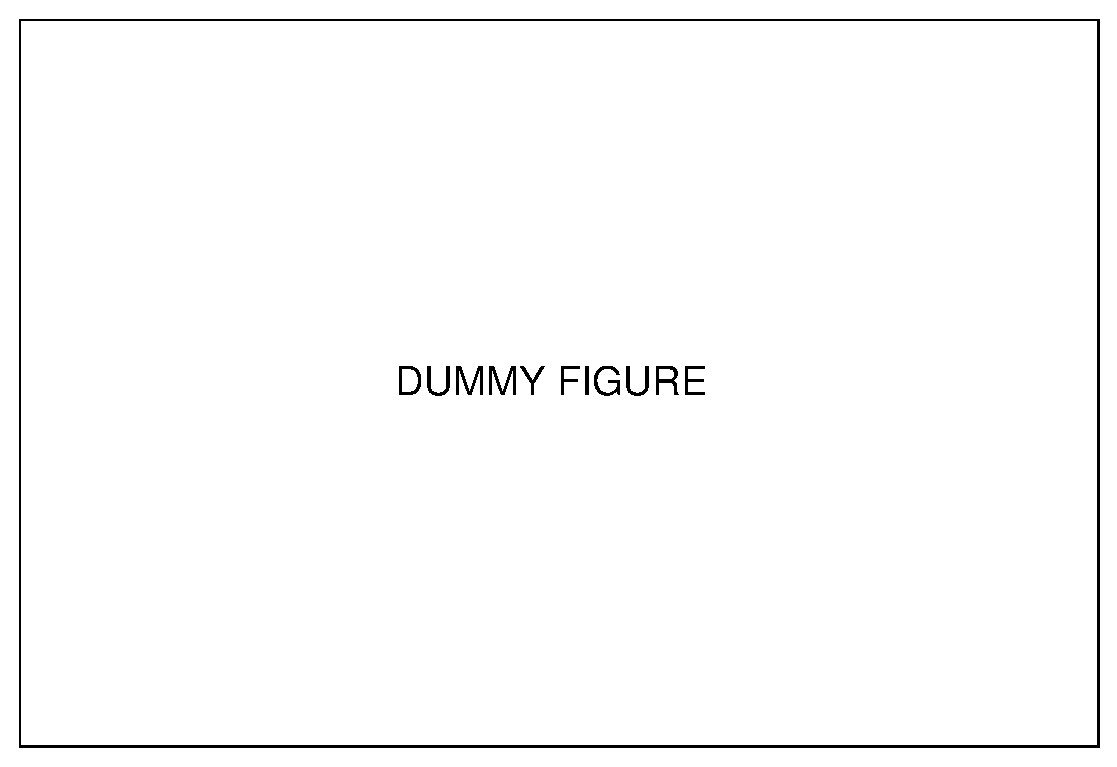
\includegraphics[width=\columnwidth,height=.7\textheight]{./figure/dummy.eps}
\end{center}
\end{center}

\item column\hfill{}\textsc{BMCOL}
\label{sec:org0511b46}
\begin{center}
\begin{center}
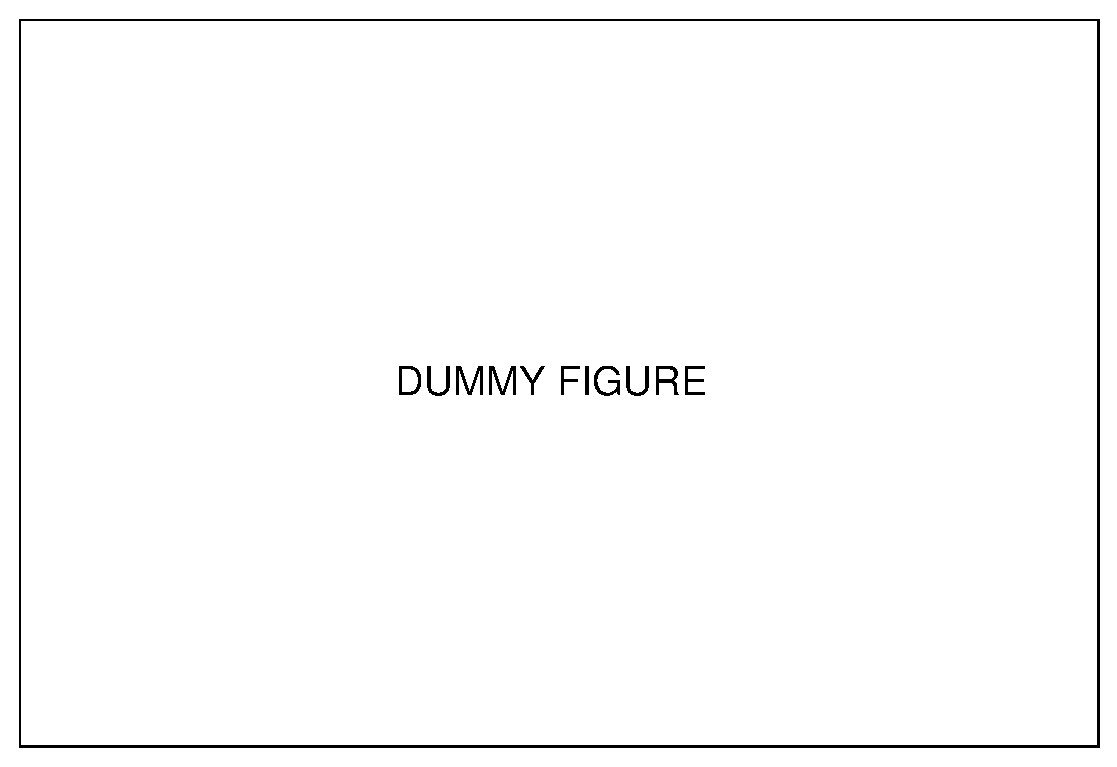
\includegraphics[width=\columnwidth,height=.7\textheight]{./figure/dummy.eps}
\end{center}
\end{center}
\end{enumerate}

\section{まとめ}
\label{sec:orgb176bab}

\subsection{まとめ}
\label{sec:orgd4af35c}

\begin{itemize}
\item あれをした
\item これをした
\end{itemize}

\subsection{今後の課題}
\label{sec:org85c2ab4}

\begin{itemize}
\item あれをしたい
\item これをしたい
\end{itemize}
\end{document}